\section{Tracing}

Another section. This one will have a figure. See
Figure~\ref{fig:us-versus-them}. Each figure has a label, which must be
defined \emph{after} the caption. Traditionally, people use
\texttt{fig:...} for figure labels, \texttt{sec:...} for section
labels, and \texttt{tab:...} for table labels. For example, this is a
reference to Section~\ref{sec:intro}. 

\begin{comment}
\begin{figure}
\centering
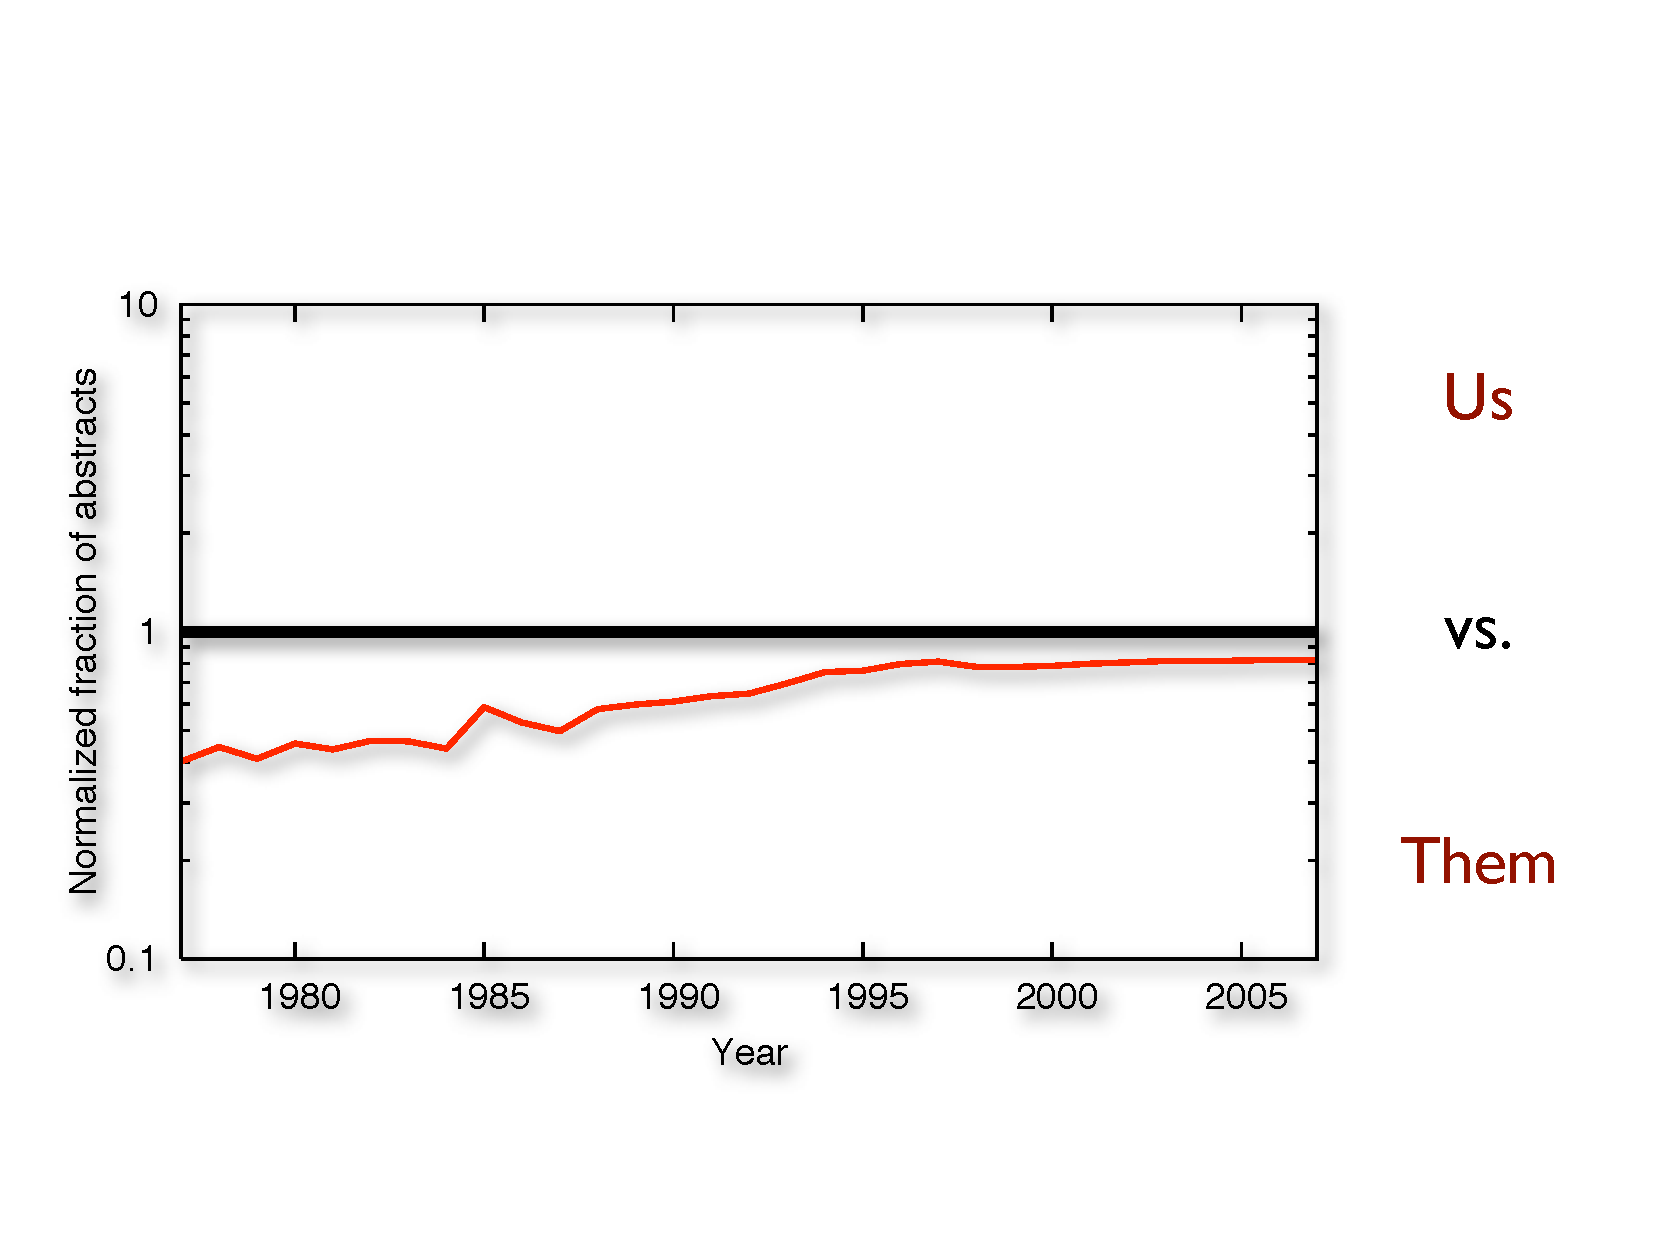
\includegraphics[width=0.7\textwidth]{usthem}
\caption{Relative number of abstracts from the ACM Digital Library
containing the word `us' versus the word 'them'. According
to~\cite{godfrey08}, `they are winning, but we are gaining on Them'. }
\label{fig:us-versus-them}
\end{figure}
\end{comment}
